% Options for packages loaded elsewhere
\PassOptionsToPackage{unicode}{hyperref}
\PassOptionsToPackage{hyphens}{url}
\documentclass[
  english,
  man,floatsintext]{apa6}
\usepackage{xcolor}
\usepackage{amsmath,amssymb}
\setcounter{secnumdepth}{-\maxdimen} % remove section numbering
\usepackage{iftex}
\ifPDFTeX
  \usepackage[T1]{fontenc}
  \usepackage[utf8]{inputenc}
  \usepackage{textcomp} % provide euro and other symbols
\else % if luatex or xetex
  \usepackage{unicode-math} % this also loads fontspec
  \defaultfontfeatures{Scale=MatchLowercase}
  \defaultfontfeatures[\rmfamily]{Ligatures=TeX,Scale=1}
\fi
\usepackage{lmodern}
\ifPDFTeX\else
  % xetex/luatex font selection
\fi
% Use upquote if available, for straight quotes in verbatim environments
\IfFileExists{upquote.sty}{\usepackage{upquote}}{}
\IfFileExists{microtype.sty}{% use microtype if available
  \usepackage[]{microtype}
  \UseMicrotypeSet[protrusion]{basicmath} % disable protrusion for tt fonts
}{}
\makeatletter
\@ifundefined{KOMAClassName}{% if non-KOMA class
  \IfFileExists{parskip.sty}{%
    \usepackage{parskip}
  }{% else
    \setlength{\parindent}{0pt}
    \setlength{\parskip}{6pt plus 2pt minus 1pt}}
}{% if KOMA class
  \KOMAoptions{parskip=half}}
\makeatother
% Make \paragraph and \subparagraph free-standing
\makeatletter
\ifx\paragraph\undefined\else
  \let\oldparagraph\paragraph
  \renewcommand{\paragraph}{
    \@ifstar
      \xxxParagraphStar
      \xxxParagraphNoStar
  }
  \newcommand{\xxxParagraphStar}[1]{\oldparagraph*{#1}\mbox{}}
  \newcommand{\xxxParagraphNoStar}[1]{\oldparagraph{#1}\mbox{}}
\fi
\ifx\subparagraph\undefined\else
  \let\oldsubparagraph\subparagraph
  \renewcommand{\subparagraph}{
    \@ifstar
      \xxxSubParagraphStar
      \xxxSubParagraphNoStar
  }
  \newcommand{\xxxSubParagraphStar}[1]{\oldsubparagraph*{#1}\mbox{}}
  \newcommand{\xxxSubParagraphNoStar}[1]{\oldsubparagraph{#1}\mbox{}}
\fi
\makeatother
\usepackage{graphicx}
\makeatletter
\newsavebox\pandoc@box
\newcommand*\pandocbounded[1]{% scales image to fit in text height/width
  \sbox\pandoc@box{#1}%
  \Gscale@div\@tempa{\textheight}{\dimexpr\ht\pandoc@box+\dp\pandoc@box\relax}%
  \Gscale@div\@tempb{\linewidth}{\wd\pandoc@box}%
  \ifdim\@tempb\p@<\@tempa\p@\let\@tempa\@tempb\fi% select the smaller of both
  \ifdim\@tempa\p@<\p@\scalebox{\@tempa}{\usebox\pandoc@box}%
  \else\usebox{\pandoc@box}%
  \fi%
}
% Set default figure placement to htbp
\def\fps@figure{htbp}
\makeatother
% definitions for citeproc citations
\NewDocumentCommand\citeproctext{}{}
\NewDocumentCommand\citeproc{mm}{%
  \begingroup\def\citeproctext{#2}\cite{#1}\endgroup}
\makeatletter
 % allow citations to break across lines
 \let\@cite@ofmt\@firstofone
 % avoid brackets around text for \cite:
 \def\@biblabel#1{}
 \def\@cite#1#2{{#1\if@tempswa , #2\fi}}
\makeatother
\newlength{\cslhangindent}
\setlength{\cslhangindent}{1.5em}
\newlength{\csllabelwidth}
\setlength{\csllabelwidth}{3em}
\newenvironment{CSLReferences}[2] % #1 hanging-indent, #2 entry-spacing
 {\begin{list}{}{%
  \setlength{\itemindent}{0pt}
  \setlength{\leftmargin}{0pt}
  \setlength{\parsep}{0pt}
  % turn on hanging indent if param 1 is 1
  \ifodd #1
   \setlength{\leftmargin}{\cslhangindent}
   \setlength{\itemindent}{-1\cslhangindent}
  \fi
  % set entry spacing
  \setlength{\itemsep}{#2\baselineskip}}}
 {\end{list}}
\usepackage{calc}
\newcommand{\CSLBlock}[1]{\hfill\break\parbox[t]{\linewidth}{\strut\ignorespaces#1\strut}}
\newcommand{\CSLLeftMargin}[1]{\parbox[t]{\csllabelwidth}{\strut#1\strut}}
\newcommand{\CSLRightInline}[1]{\parbox[t]{\linewidth - \csllabelwidth}{\strut#1\strut}}
\newcommand{\CSLIndent}[1]{\hspace{\cslhangindent}#1}
\ifLuaTeX
\usepackage[bidi=basic]{babel}
\else
\usepackage[bidi=default]{babel}
\fi
% get rid of language-specific shorthands (see #6817):
\let\LanguageShortHands\languageshorthands
\def\languageshorthands#1{}
\ifLuaTeX
  \usepackage[english]{selnolig} % disable illegal ligatures
\fi
\setlength{\emergencystretch}{3em} % prevent overfull lines
\providecommand{\tightlist}{%
  \setlength{\itemsep}{0pt}\setlength{\parskip}{0pt}}
% Manuscript styling
\usepackage{upgreek}
\captionsetup{font=singlespacing,justification=justified}

% Table formatting
\usepackage{longtable}
\usepackage{lscape}
% \usepackage[counterclockwise]{rotating}   % Landscape page setup for large tables
\usepackage{multirow}		% Table styling
\usepackage{tabularx}		% Control Column width
\usepackage[flushleft]{threeparttable}	% Allows for three part tables with a specified notes section
\usepackage{threeparttablex}            % Lets threeparttable work with longtable

% Create new environments so endfloat can handle them
% \newenvironment{ltable}
%   {\begin{landscape}\centering\begin{threeparttable}}
%   {\end{threeparttable}\end{landscape}}
\newenvironment{lltable}{\begin{landscape}\centering\begin{ThreePartTable}}{\end{ThreePartTable}\end{landscape}}

% Enables adjusting longtable caption width to table width
% Solution found at http://golatex.de/longtable-mit-caption-so-breit-wie-die-tabelle-t15767.html
\makeatletter
\newcommand\LastLTentrywidth{1em}
\newlength\longtablewidth
\setlength{\longtablewidth}{1in}
\newcommand{\getlongtablewidth}{\begingroup \ifcsname LT@\roman{LT@tables}\endcsname \global\longtablewidth=0pt \renewcommand{\LT@entry}[2]{\global\advance\longtablewidth by ##2\relax\gdef\LastLTentrywidth{##2}}\@nameuse{LT@\roman{LT@tables}} \fi \endgroup}

% \setlength{\parindent}{0.5in}
% \setlength{\parskip}{0pt plus 0pt minus 0pt}

% Overwrite redefinition of paragraph and subparagraph by the default LaTeX template
% See https://github.com/crsh/papaja/issues/292
\makeatletter
\renewcommand{\paragraph}{\@startsection{paragraph}{4}{\parindent}%
  {0\baselineskip \@plus 0.2ex \@minus 0.2ex}%
  {-1em}%
  {\normalfont\normalsize\bfseries\itshape\typesectitle}}

\renewcommand{\subparagraph}[1]{\@startsection{subparagraph}{5}{1em}%
  {0\baselineskip \@plus 0.2ex \@minus 0.2ex}%
  {-\z@\relax}%
  {\normalfont\normalsize\itshape\hspace{\parindent}{#1}\textit{\addperi}}{\relax}}
\makeatother

\makeatletter
\usepackage{etoolbox}
\patchcmd{\maketitle}
  {\section{\normalfont\normalsize\abstractname}}
  {\section*{\normalfont\normalsize\abstractname}}
  {}{\typeout{Failed to patch abstract.}}
\patchcmd{\maketitle}
  {\section{\protect\normalfont{\@title}}}
  {\section*{\protect\normalfont{\@title}}}
  {}{\typeout{Failed to patch title.}}
\makeatother

\usepackage{xpatch}
\makeatletter
\xapptocmd\appendix
  {\xapptocmd\section
    {\addcontentsline{toc}{section}{\appendixname\ifoneappendix\else~\theappendix\fi: #1}}
    {}{\InnerPatchFailed}%
  }
{}{\PatchFailed}
\makeatother
\keywords{manifestos, harm, justification, political\newline\indent Word count: X}
\usepackage{csquotes}
\usepackage{placeins}
\usepackage{flafter}
\usepackage{bookmark}
\IfFileExists{xurl.sty}{\usepackage{xurl}}{} % add URL line breaks if available
\urlstyle{same}
\hypersetup{
  pdftitle={Justifications of Dyadic Harm in Political Manifestos},
  pdfauthor={Morgan Ballesteros},
  pdflang={en-EN},
  pdfkeywords={manifestos, harm, justification, political},
  hidelinks,
  pdfcreator={LaTeX via pandoc}}

\title{\textbf{Justifications of Dyadic Harm in Political Manifestos}}
\author{Morgan Ballesteros\textsuperscript{}}
\date{}


\shorttitle{Justifying Dyadic Harm}

\authornote{

Correspondence concerning this article should be addressed to Morgan Ballesteros. E-mail: \href{mailto:mballesteros@uchicago.edu}{\nolinkurl{mballesteros@uchicago.edu}}

}

\affiliation{\vspace{0.5cm}\textsuperscript{} University of Chicago}

\begin{document}
\maketitle

The theory of dyadic morality suggests that judgments of harm give moral valence to
relationships between an intentional agent and vulnerable patient (Schein \& Gray, 2018).
That is, dyadic morality predicts that if one were to see someone (i.e., an agent) intentionally harming another person (i.e., a vulnerable patient), one would judge that this action (i.e., the harming of another person) is immoral or morally wrong. Furthermore, social interactions are composed of moral norms as mutually agreed upon rules as to how citizens ought to behave. Although moral norms (e.g., do not murder) are meant to keep people from damaging others, some justify norm violations --- and harm --- in pursuit of a goal (e.g., political assassinations), whereas others never condone violence to induce change. Understanding what differentiates violent and non-violent agents is therefore useful in protecting against harmful acts. One source that marks such differences is the political manifesto (i.e., ``a written statement declaring publicly the intentions, motives, or views of its issuer''; Merriam-Webster, n.d.). The current study targets differences in linguistic indicators of justifications of harm and integrative complexity between violence-condoning and non-violent manifestos.\\
Research on linguistic markers of political violence follows the growing number of far-right
manifestos published online prior to terrorist attacks (Capelos, DaVisio, \& Salmela, 2025; Ebner, Kavanagh, \& Whitehouse, 2025). Some of these studies evaluate manifestos through the fusion-plus-threat model of
violent extremism (Whitehouse, 2018), which predicts that individuals who lump their personal
and group identities together will be more likely to self-sacrifice for their group.
Associated linguistic work suggests that words indicating identity fusion, group threat, and
violence-condoning norms --- including justifications of violence --- are correlated with
terrorism (Ebner, Kavanagh, \& Whitehouse, 2024; Ebner et al., 2025). While the existing literature grounds the
importance of justificatory rhetoric in predicting terrorism, harm has not yet been examined
as central to moral judgment despite its importance in some theories of moral judgment (e.g.,
the theory of dyadic morality). The present study serves as a real-world case on how emotion
and reason interact to produce the judgments and justifications necessary for enacting harm.
Connecting the political manifesto and moral judgment literatures will enlighten respective
research as to (a) how moral reasoning implicates justification in manifestos and (b) how
justification operates in the moral reasoning process, each of which could have policy
implications.\\
Integrative Complexity is a linguistic measure of cognitive complexity composed of two primary components: (a) Differentiation and (b) Integration (Suedfeld, Tetlock, \& Streufert, 1992). Differentiation indicates how many perspectives one accounts for; Integration indicates the extent to which those differentiated perspectives are synthesized. A useful example is an argumentative essay, which, if it is complex, recognizes a variety of possible arguments for or against some claim, and synthesizes those arguments into one ultimate argument, using parts of each subsidiary argument (Ballesteros, 2025). Integrative complexity shows a robust relationship with political violence (Suedfeld, 2010). However, research using the construct as a predictor of political violence has largely focused on political leaders in respect to events like war and international crises (Suedfeld, 2010). To my knowledge, no study to date has directly linked the integrative complexity of political manifestos with justifications of political violence. Considering the measure's long-standing precedent in predicting political events, integrating integrative complexity into the manifesto literature could help identify the factors that distinguish between merely violent rhetoric and rhetoric that induces violence, thereby affording greater predictability through an aggregation of said factors.

\subsection{Current Study}\label{current-study}

The current study contributes to research seeking to identify differences between violent and non-violent political agents through an evaluation of political manifestos in two new ways: (a) by focusing a qualitative analysis on rhetoric about harm as designating moral valence by the theory of dyadic morality and (b) by scoring manifestos on integrative complexity. I seek to aid in answering three related questions: (a) do justifications of harm correspond to changes in individual moral norms?; (b) does integrative complexity predict whether a manifesto will result in violence versus non-violence?; and (c) does integrative complexity predict both temporally near and far instances of violence in relation to political manifestos? I predict that (a) changes in moral norms --- as exemplified in the agents' writings --- and subsequent justification of increasingly harmful acts will be associated with a higher likelihood of violence, (b) lower levels of integrative complexity in political manifestos will predict higher likelihoods of violence, and (c) a decrease in integrative complexity will be associated with an individual coming to believe that harm is justified in pursuit of their political goals.

\section{Method}\label{method}

\subsection{Manifesto Selection}\label{manifesto-selection}

This study includes manifestos divided into three categories following Ebner et al. (2025); (a) violent self-sacrificial, (b) ideologically extreme, and (c) moderate. It also affords longitudinal analysis. I selected not only one-off manifestos already analyzed in the aforementioned literature (e.g., Anders Behring Breivik's Manifesto of the Norway Attacks, 2011; Marx \& Engels Manifesto of the Communist Party, 1848), but also sets of writings of individual authors across time (e.g., selections of Vladimir Lenin's letters). Materials include ten manifestos for each of the aforementioned categories, and three longitudinal sets of writings for each category. Incorporating the 15 manifestos previously analyzed in the literature brings the study to a categorical count as follows: (a) nine violent self-sacrificial texts, (b) three ideologically extreme texts, and (c) 3 moderate texts. Each of these texts are one-off samples. To fill out the rest of the ten one-off samples for each category, manifestos were selected according to their place on the political spectrum (i.e., left to right political platforms), individual actor-author texts versus platform-representative texts, and length in order to match each category along these factors. The same factors were considered in choosing longitudinal samples, and selection included qualitatively matching samples across categories.

\subsection{Measures}\label{measures}

\subsubsection{Linguistic Indicators}\label{linguistic-indicators}

Ebner et al. (2025) supplies a list of words that indicate
justifications of violence and, as a higher-order category of linguistic markers, violence
condoning norms. The current study uses the set of words indicating violence condoning
norms with minor alterations. First, indicators like ``need for jihaad'' (Ebner et al., 2025)
have been replaced with relevant phrasing (e.g., need for war; need for revolution). Second,
specific indicators of talk about harm in dyadic morality (e.g., harm, damage, agent,
patient, intentional) have been added to the list of indicators.\\

\subsubsection{Automated Integrative Complexity}\label{automated-integrative-complexity}

Hand-scoring integrative complexity is an involved
process requiring multiple scorers and often hours of work per scored material. In light of
time and manpower limitations, this study instead uses automated integrative complexity
(Conway, Conway, Gornick, \& Houck, 2014) to score materials, a measure that uses linguistic markers of
differentiation and integration to construct an automated account of integrative complexity.
While automated integrative complexity does not correlate perfectly with hand scores
(document-level correlation of .82, paragraph-level correlation of .46, Conway, Conway, \& Houck, 2020), it is an increasingly validated measure in its own right and often used as an
efficient and effective replacement for hand scoring. This study uses the document-level
scores for all analyses.

\subsubsection{Violence}\label{violence}

Previously analyzed manifestos are easily delineated as to whether they cause
violence; some manifestos precede lone-actor attacks by their author, the other manifestos
did not precede violence enacted by their author. The present study maintains this
distinction. However, it also includes platform-based violence by identifying institutional
violence in direct causal relationship with the philosophies put forward by corresponding
manifestos. For example, a manifesto by a political leader that accompanies a war (e.g., the
\emph{Russian Imperial Manifesto of 1914} by Tzar Nicholas II announcing Russia's entry into World
War One; Golder, 1927) would be counted as violent; a manifesto espoused by a political
leader that does not accompany institutional violence by that leader's institution (e.g.,
John F. Kennedy's \emph{Ich bin ein Berliner}) would be counted as non-violent.

\subsubsection{Analyses}\label{analyses}

Following Ebner et al. (2024), I measure the prevalence of each linguistic marker group as occurrences per 1,000 words (word-count--normalized rates). Marker groups include dyadic harm language (added to reflect dyadic morality), justification for violence, martyrdom narratives, hopelessness of alternatives, role model status, and violent references.\\
To test whether these linguistic indicators differ across manifesto categories (moderate, ideologically extreme, violent self-sacrificial), I estimate linear models predicting each marker group's prevalence from category and report category means with confidence intervals.\\
To directly test the hypothesis that integrative complexity predicts violence versus non-violence, I estimate logistic regression models predicting whether a manifesto is classified as violent (vs.~non-violent) from document-level AutoIC integrative complexity scores (and, in expanded models, from the marker-group prevalence measures).\\
For longitudinal corpora (multiple texts per author over time), I estimate mixed-effects regression models assessing (a) within-author changes in integrative complexity and harm-justification language over time and (b) whether lower integrative complexity is associated with higher harm-justification language within authors. Where violence event dates are available, I additionally examine whether integrative complexity and harm-justification indicators differ in texts written nearer versus farther from the violence event.

\section{Results}\label{results}

\begin{verbatim}
## n used by lm after na.omit = 264
\end{verbatim}

\begin{verbatim}
## category distribution in modeling data:
\end{verbatim}

\begin{verbatim}
## 
## moderate  extreme  violent 
##       95      125       44
\end{verbatim}

\begin{verbatim}
## 
## Call:
## lm(formula = form_ic2, data = mf)
## 
## Residuals:
##     Min      1Q  Median      3Q     Max 
## -1.1518 -0.1988 -0.0299  0.1662  3.3723 
## 
## Coefficients:
##                             Estimate Std. Error t value Pr(>|t|)    
## (Intercept)                 1.999894   0.056769  35.228   <2e-16 ***
## dyadic_harm                 0.176825   0.078387   2.256   0.0249 *  
## hopelessness               -0.005058   0.005790  -0.874   0.3832    
## justification_for_violence -0.041855   0.036109  -1.159   0.2475    
## martyrdom_narrative        -0.012110   0.063300  -0.191   0.8484    
## role_model_status          -0.018937   0.033540  -0.565   0.5728    
## violent_reference          -0.039219   0.055904  -0.702   0.4836    
## categoryextreme             0.151942   0.063411   2.396   0.0173 *  
## categoryviolent             0.034667   0.081026   0.428   0.6691    
## ---
## Signif. codes:  0 '***' 0.001 '**' 0.01 '*' 0.05 '.' 0.1 ' ' 1
## 
## Residual standard error: 0.4169 on 255 degrees of freedom
## Multiple R-squared:  0.05528,    Adjusted R-squared:  0.02564 
## F-statistic: 1.865 on 8 and 255 DF,  p-value: 0.06588
\end{verbatim}

\subsection{Descriptive Statistics}\label{descriptive-statistics}

\begin{figure}
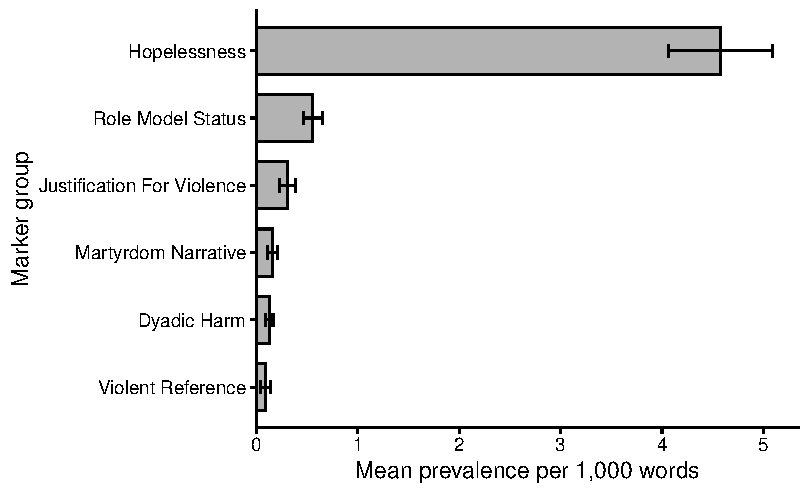
\includegraphics[width=0.82\linewidth]{Thesis_files/figure-latex/group-prevalence-plot-1} \caption{Mean prevalence of grouped linguistic indicators of harm justification. Note. Bars represent mean grouped marker prevalence per 1,000 words across documents. Error bars represent 95\% confidence intervals. Marker groups aggregate lexical indicators defined in the study's marker dictionary.}\label{fig:group-prevalence-plot}
\end{figure}

Descriptive statistics were calculated to examine the prevalence of grouped linguistic indicators of harm justification across the manifesto corpus. Prevalence values represent occurrences of grouped markers per 1,000 words. Across all 267 manifestos, markers associated with hopelessness were the most common (M = 4.58, SD = 4.59), followed by role model status (M = 0.56, SD = 0.83), justification for violence (M = 0.31, SD = 0.71), martyrdom narratives (M = 0.16, SD = 0.45), dyadic harm language (M = 0.13, SD = 0.33), and references to violent actors or events (M = 0.09, SD = 0.45). Minimum and maximum prevalence values ranged from 0 to 31.21 depending on marker group.

\begin{table}[tbp]

\begin{center}
\begin{threeparttable}

\caption{\label{tab:manifesto-descriptives}Mean prevalence of grouped linguistic indicators by manifesto category.}

\begin{tabular}{llll}
\toprule
Marker Group & \multicolumn{1}{c}{moderate} & \multicolumn{1}{c}{extreme} & \multicolumn{1}{c}{violent}\\
\midrule
Dyadic Harm & 0.13 & 0.07 & 0.32\\
Justification for Violence & 0.53 & 0.20 & 0.22\\
Martyrdom Narrative & 0.13 & 0.17 & 0.21\\
Hopelessness & 3.02 & 5.76 & 3.62\\
\bottomrule
\addlinespace
\end{tabular}

\begin{tablenotes}[para]
\normalsize{\textit{Note.} Values represent grouped marker prevalence per 1,000 words.}
\end{tablenotes}

\end{threeparttable}
\end{center}

\end{table}

Mean marker prevalence also differed across manifesto categories (Table \ref{tab:manifesto-descriptives}). Violent self-sacrificial manifestos exhibited the highest average prevalence of dyadic harm language (M = 0.32) and justification for violence (M = 0.22), whereas moderate manifestos displayed very low levels of these indicators (dyadic harm M = 0.13; justification for violence M = 0.53). Martyrdom narratives showed the most pronounced difference across categories, appearing most frequently in violent manifestos (M = 0.21) compared with extreme (M = 0.17) and moderate texts (M = 0.13). In contrast, markers associated with hopelessness were most prevalent in ideologically extreme manifestos (M = 5.76), followed by moderate manifestos (M = 3.02) and violent manifestos (M = 3.62).

\subsection{Regression Analyses}\label{regression-analyses}

To examine whether manifesto category predicts the prevalence of harm-related linguistic indicators, a series of linear regression models were estimated. Each model predicted the prevalence of a marker group from manifesto category, with moderate manifestos serving as the reference category.

\subsubsection{Dyadic Harm Language}\label{dyadic-harm-language}

The overall model approached significance, F(2, 28) = 3.10, p = .061, R² = .18. Relative to moderate manifestos, both ideologically extreme (b = 0.16, SE = 0.08, p = .040) and violent manifestos (b = 0.18, SE = 0.08, p = .035) exhibited significantly higher levels of dyadic harm language.

\subsubsection{Justifications for Violence}\label{justifications-for-violence}

The model was not significant, F(2, 28) = 1.88, p = .171, R² = .12. Neither ideologically extreme (p = .744) nor violent manifestos (p = .085) differed significantly from moderate texts, although the latter showed a trend toward higher prevalence.

\subsubsection{Martyrdom Narratives}\label{martyrdom-narratives}

The model was significant, F(2, 28) = 3.94, p = .031, R² = .22. Violent manifestos exhibited higher levels of martyrdom language than moderate texts (b = 0.47, SE = 0.19, p = .019), whereas ideologically extreme manifestos did not differ from moderate texts (p = .780).

\subsubsection{Hopelessness}\label{hopelessness}

The model was not significant, F(2, 28) = 2.48, p = .102, R² = .15. No category differences were observed.

\subsubsection{Integrative Complexity Predicting Violence}\label{integrative-complexity-predicting-violence}

Logistic regression models assessed whether integrative complexity predicted whether a manifesto was classified as violent (vs.~non-violent; see Tables 2--3). In the baseline model, integrative complexity was negatively associated with violence likelihood, OR = 0.13, 95\% CI {[}0.01, 0.91{]}, p = .079. In the full model including linguistic indicators, integrative complexity remained a significant predictor, OR = 0.04, 95\% CI {[}0.00, 0.69{]}, p = .050.

Among linguistic predictors, martyrdom narratives (OR = 14.63, p = .060) and justification for violence (OR = 4.05, p = .084) showed large but non-significant effects. Dyadic harm language and hopelessness did not significantly predict violence when included in the full model.

A multinomial logistic regression model was estimated as a sensitivity analysis to examine whether predictors differentiated across all three manifesto categories (Table 4). Results were broadly consistent with the binary logistic models, with lower integrative complexity associated with greater likelihood of classification in more extreme categories relative to moderate texts. However, estimates were highly unstable, with large relative risk ratios and wide confidence intervals, limiting interpretability.

\begin{table}[tbp]

\begin{center}
\begin{threeparttable}

\caption{\label{tab:violent-logistic-models}Logistic regression predicting violent (vs. non-violent) category from integrative complexity.}

\begin{tabular}{llll}
\toprule
Predictor & \multicolumn{1}{c}{OR} & \multicolumn{1}{c}{CI} & \multicolumn{1}{c}{p}\\
\midrule
Integrative Complexity (z) & 1.01 & {}[0.74, 1.4] & 0.928\\
\bottomrule
\addlinespace
\end{tabular}

\begin{tablenotes}[para]
\normalsize{\textit{Note.} Odds ratios (OR), 95\% confidence intervals, and p values are Wald-based. OR reflects a 1 SD increase in standardized integrative complexity.}
\end{tablenotes}

\end{threeparttable}
\end{center}

\end{table}

\begin{table}[tbp]

\begin{center}
\begin{threeparttable}

\caption{\label{tab:violent-logistic-models}Logistic regression predicting violent (vs. non-violent) manifesto category from integrative complexity and linguistic indicators.}

\begin{tabular}{llll}
\toprule
Predictor & \multicolumn{1}{c}{OR} & \multicolumn{1}{c}{CI} & \multicolumn{1}{c}{p}\\
\midrule
Integrative Complexity (z) & 0.89 & {}[0.61, 1.28] & 0.521\\
Dyadic Harm (z) & 1.97 & {}[1.37, 2.84] & < .001\\
Justification for Violence (z) & 0.53 & {}[0.27, 1.03] & 0.061\\
Martyrdom Narrative (z) & 1.17 & {}[0.88, 1.54] & 0.282\\
Hopelessness (z) & 0.62 & {}[0.4, 0.96] & 0.034\\
\bottomrule
\addlinespace
\end{tabular}

\begin{tablenotes}[para]
\normalsize{\textit{Note.} Odds ratios (OR), 95\% confidence intervals, and p values are Wald-based. OR reflects a 1 SD increase in each standardized predictor.}
\end{tablenotes}

\end{threeparttable}
\end{center}

\end{table}

\begin{table}[tbp]

\begin{center}
\begin{threeparttable}

\caption{\label{tab:violent-logistic-models}Reduced logistic models predicting violent (vs. non-violent) category from individual predictors.}

\begin{tabular}{llll}
\toprule
Model & \multicolumn{1}{c}{OR} & \multicolumn{1}{c}{CI} & \multicolumn{1}{c}{p}\\
\midrule
IC only & 1.01 & {}[0.74, 1.40] & 0.928\\
Dyadic Harm only & 1.62 & {}[1.20, 2.18] & 0.002\\
Justification only & 0.73 & {}[0.42, 1.28] & 0.276\\
Hopelessness only & 0.73 & {}[0.48, 1.11] & 0.137\\
\bottomrule
\end{tabular}

\end{threeparttable}
\end{center}

\end{table}

\begin{figure}
\centering
\pandocbounded{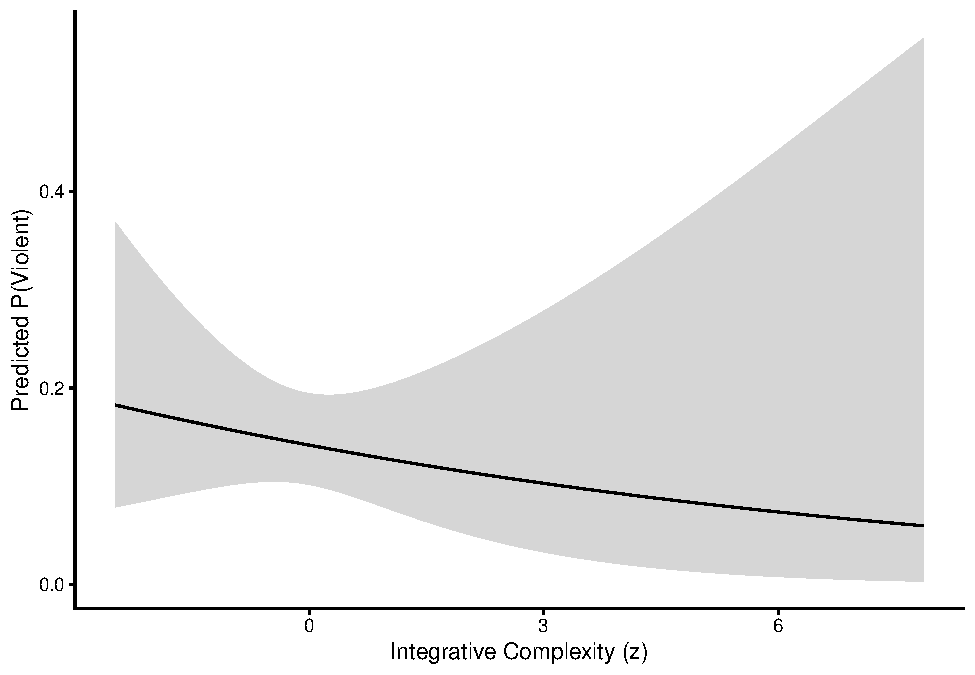
\includegraphics[keepaspectratio]{Thesis_files/figure-latex/fig-violent-probability-1.pdf}}
\caption{\label{fig:fig-violent-probability}Predicted probability of violent (vs.~non-violent) category as a function of integrative complexity (95\% CI).}
\end{figure}

\begin{figure}
\centering
\pandocbounded{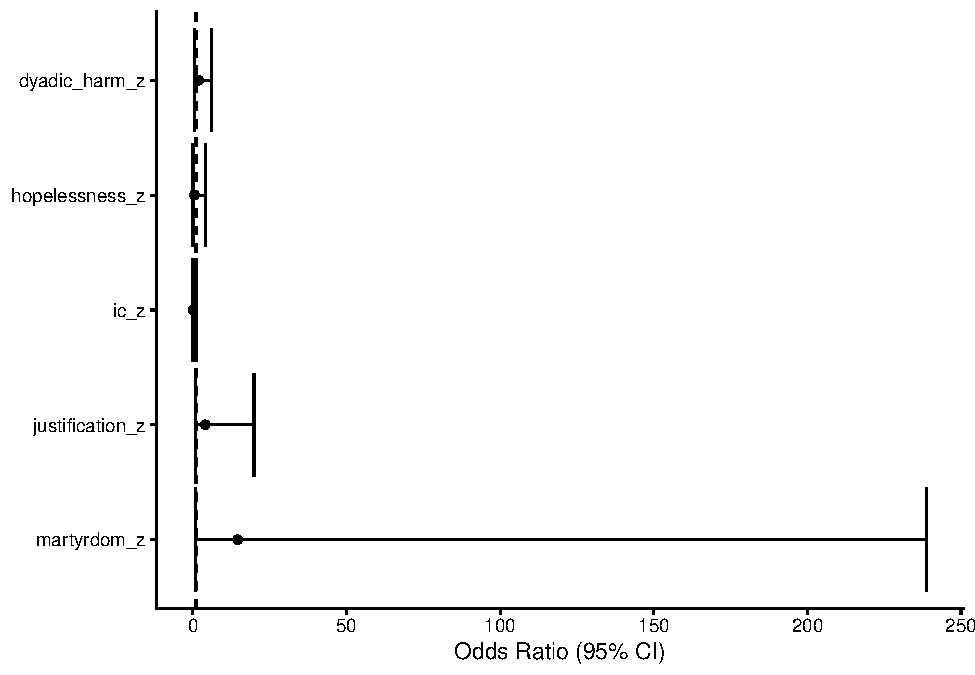
\includegraphics[keepaspectratio]{Thesis_files/figure-latex/fig-violent-oddsratios-1.pdf}}
\caption{\label{fig:fig-violent-oddsratios}Odds ratios (95\% CI) from the logistic model predicting violent (vs.~non-violent) category.}
\end{figure}

\begin{verbatim}
## [1] 0.0003014245 0.9593271053
\end{verbatim}

\begin{verbatim}
##    Min. 1st Qu.  Median    Mean 3rd Qu.    Max. 
## -1.4798 -0.6154 -0.5038 -0.1717 -0.3666  2.7156
\end{verbatim}

\begin{verbatim}
##      Min.   1st Qu.    Median      Mean   3rd Qu.      Max. 
## 1.700e-07 1.876e-04 3.067e-04 7.644e-03 1.419e-03 3.929e-01
\end{verbatim}

\begin{table}[tbp]

\begin{center}
\begin{threeparttable}

\caption{\label{tab:marker-group-regressions}Linear regression coefficients predicting grouped marker prevalence from manifesto category.}

\begin{tabular}{llllll}
\toprule
Outcome & \multicolumn{1}{c}{Contrast} & \multicolumn{1}{c}{B} & \multicolumn{1}{c}{SE} & \multicolumn{1}{c}{t} & \multicolumn{1}{c}{p}\\
\midrule
Dyadic Harm & Extreme vs. Moderate & -0.06 & 0.04 & -1.44 & 0.152\\
Dyadic Harm & Violent vs. Moderate & 0.19 & 0.06 & 3.24 & 0.001\\
Justification & Extreme vs. Moderate & -0.33 & 0.09 & -3.71 & < .001\\
Justification & Violent vs. Moderate & -0.31 & 0.13 & -2.47 & 0.014\\
Martyrdom & Extreme vs. Moderate & 0.04 & 0.06 & 0.72 & 0.470\\
Martyrdom & Violent vs. Moderate & 0.08 & 0.08 & 0.95 & 0.343\\
Hopelessness & Extreme vs. Moderate & 2.74 & 0.57 & 4.79 & < .001\\
Hopelessness & Violent vs. Moderate & 0.60 & 0.81 & 0.74 & 0.458\\
\bottomrule
\addlinespace
\end{tabular}

\begin{tablenotes}[para]
\normalsize{\textit{Note.} Moderate manifestos served as the reference category.}
\end{tablenotes}

\end{threeparttable}
\end{center}

\end{table}

\begin{table}[tbp]

\begin{center}
\begin{threeparttable}

\caption{\label{tab:manifesto-regressions}Linear regression coefficients predicting document-level autoIC outcomes from linguistic indicators and manifesto category.}

\begin{tabular}{llllll}
\toprule
Outcome & \multicolumn{1}{c}{Predictor} & \multicolumn{1}{c}{B} & \multicolumn{1}{c}{SE} & \multicolumn{1}{c}{t} & \multicolumn{1}{c}{p}\\
\midrule
IC & Justification for Violence & -0.05 & 0.04 & -1.34 & 0.182\\
IC & Dyadic Harm & 0.17 & 0.08 & 2.18 & 0.030\\
IC & Extreme vs. Moderate & 0.15 & 0.06 & 2.58 & 0.010\\
IC & Violent vs. Moderate & 0.05 & 0.08 & 0.59 & 0.553\\
Dial & Justification for Violence & -0.01 & 0.03 & -0.37 & 0.708\\
Dial & Dyadic Harm & 0.15 & 0.06 & 2.57 & 0.011\\
Dial & Extreme vs. Moderate & 0.10 & 0.04 & 2.22 & 0.027\\
Dial & Violent vs. Moderate & 0.14 & 0.06 & 2.38 & 0.018\\
Elab & Justification for Violence & -0.03 & 0.02 & -1.18 & 0.238\\
Elab & Dyadic Harm & 0.04 & 0.05 & 0.78 & 0.433\\
Elab & Extreme vs. Moderate & 0.04 & 0.04 & 1.17 & 0.242\\
Elab & Violent vs. Moderate & 0.02 & 0.05 & 0.30 & 0.766\\
IC Differentiation & Justification for Violence & -0.01 & 0.02 & -0.35 & 0.725\\
IC Differentiation & Dyadic Harm & 0.08 & 0.05 & 1.57 & 0.117\\
IC Differentiation & Extreme vs. Moderate & 0.05 & 0.04 & 1.29 & 0.200\\
IC Differentiation & Violent vs. Moderate & 0.16 & 0.05 & 3.05 & 0.003\\
IC Integration & Justification for Violence & -0.04 & 0.02 & -1.70 & 0.090\\
IC Integration & Dyadic Harm & 0.08 & 0.05 & 1.74 & 0.083\\
IC Integration & Extreme vs. Moderate & 0.09 & 0.04 & 2.57 & 0.011\\
IC Integration & Violent vs. Moderate & -0.12 & 0.05 & -2.38 & 0.018\\
Dial Differentiation & Justification for Violence & 0.01 & 0.02 & 0.41 & 0.679\\
Dial Differentiation & Dyadic Harm & 0.07 & 0.05 & 1.53 & 0.127\\
Dial Differentiation & Extreme vs. Moderate & 0.05 & 0.04 & 1.48 & 0.141\\
Dial Differentiation & Violent vs. Moderate & 0.20 & 0.05 & 3.97 & < .001\\
Dial Integration & Justification for Violence & -0.02 & 0.01 & -1.45 & 0.148\\
Dial Integration & Dyadic Harm & 0.08 & 0.03 & 2.68 & 0.008\\
Dial Integration & Extreme vs. Moderate & 0.04 & 0.02 & 2.04 & 0.042\\
Dial Integration & Violent vs. Moderate & -0.04 & 0.03 & -1.48 & 0.141\\
Elab Differentiation & Justification for Violence & -0.01 & 0.02 & -0.50 & 0.619\\
Elab Differentiation & Dyadic Harm & 0.03 & 0.04 & 0.79 & 0.430\\
Elab Differentiation & Extreme vs. Moderate & 0.00 & 0.03 & -0.11 & 0.911\\
Elab Differentiation & Violent vs. Moderate & 0.09 & 0.04 & 2.35 & 0.019\\
Elab Integration & Justification for Violence & -0.02 & 0.01 & -1.62 & 0.107\\
Elab Integration & Dyadic Harm & 0.01 & 0.03 & 0.23 & 0.820\\
Elab Integration & Extreme vs. Moderate & 0.04 & 0.02 & 2.15 & 0.032\\
Elab Integration & Violent vs. Moderate & -0.08 & 0.03 & -2.91 & 0.004\\
\bottomrule
\addlinespace
\end{tabular}

\begin{tablenotes}[para]
\normalsize{\textit{Note.} Moderate manifestos served as the reference category. Coefficients for linguistic predictors represent associations with document-level autoIC outcomes, controlling for the other predictors in the model.}
\end{tablenotes}

\end{threeparttable}
\end{center}

\end{table}

\begin{table}[tbp]

\begin{center}
\begin{threeparttable}

\caption{\label{tab:category-nonparametric-tests}Kruskal-Wallis tests comparing marker prevalence across manifesto categories.}

\begin{tabular}{lllllll}
\toprule
measure & \multicolumn{1}{c}{.y.} & \multicolumn{1}{c}{n} & \multicolumn{1}{c}{statistic} & \multicolumn{1}{c}{df} & \multicolumn{1}{c}{p} & \multicolumn{1}{c}{method}\\
\midrule
dyadic\_harm & value & 305 & 21.93 & 2 & 0.00 & Kruskal-Wallis\\
hopelessness & value & 305 & 41.36 & 2 & 0.00 & Kruskal-Wallis\\
justification\_for\_violence & value & 305 & 41.23 & 2 & 0.00 & Kruskal-Wallis\\
martyrdom\_narrative & value & 305 & 6.65 & 2 & 0.04 & Kruskal-Wallis\\
\bottomrule
\end{tabular}

\end{threeparttable}
\end{center}

\end{table}

\begin{table}[tbp]

\begin{center}
\begin{threeparttable}

\caption{\label{tab:category-nonparametric-tests}Pairwise Wilcoxon tests (Holm-corrected) comparing manifesto categories.}

\begin{tabular}{llllllllll}
\toprule
measure & \multicolumn{1}{c}{.y.} & \multicolumn{1}{c}{group1} & \multicolumn{1}{c}{group2} & \multicolumn{1}{c}{n1} & \multicolumn{1}{c}{n2} & \multicolumn{1}{c}{statistic} & \multicolumn{1}{c}{p} & \multicolumn{1}{c}{p.adj} & \multicolumn{1}{c}{p.adj.signif}\\
\midrule
dyadic\_harm & value & moderate & extreme & 95 & 166 & 9,925.00 & 0.00 & 0.00 & ****\\
dyadic\_harm & value & moderate & violent & 95 & 44 & 2,190.00 & 0.61 & 0.61 & ns\\
dyadic\_harm & value & extreme & violent & 166 & 44 & 2,975.00 & 0.00 & 0.01 & **\\
hopelessness & value & moderate & extreme & 95 & 166 & 4,929.50 & 0.00 & 0.00 & ****\\
hopelessness & value & moderate & violent & 95 & 44 & 2,706.50 & 0.00 & 0.00 & **\\
hopelessness & value & extreme & violent & 166 & 44 & 5,420.50 & 0.00 & 0.00 & ****\\
justification\_for\_violence & value & moderate & extreme & 95 & 166 & 11,119.00 & 0.00 & 0.00 & ****\\
justification\_for\_violence & value & moderate & violent & 95 & 44 & 2,827.00 & 0.00 & 0.00 & ***\\
justification\_for\_violence & value & extreme & violent & 166 & 44 & 3,351.50 & 0.28 & 0.28 & ns\\
martyrdom\_narrative & value & moderate & extreme & 95 & 166 & 9,037.00 & 0.01 & 0.03 & *\\
martyrdom\_narrative & value & moderate & violent & 95 & 44 & 2,322.00 & 0.21 & 0.42 & ns\\
martyrdom\_narrative & value & extreme & violent & 166 & 44 & 3,488.50 & 0.52 & 0.52 & ns\\
\bottomrule
\end{tabular}

\end{threeparttable}
\end{center}

\end{table}

\subsection{Longitudinal Analyses}\label{longitudinal-analyses}

Mixed-effects models were estimated to examine within-author changes in integrative complexity and justification language over time (see Table 6; Figure 2). No significant effects were observed. Integrative complexity was not associated with justification language (b = -0.11, SE = 0.11, t = -0.99), nor did either variable change systematically over time. These findings suggest that cross-sectional differences across manifesto types are more pronounced than within-author temporal dynamics.

\begin{figure}
\centering
\pandocbounded{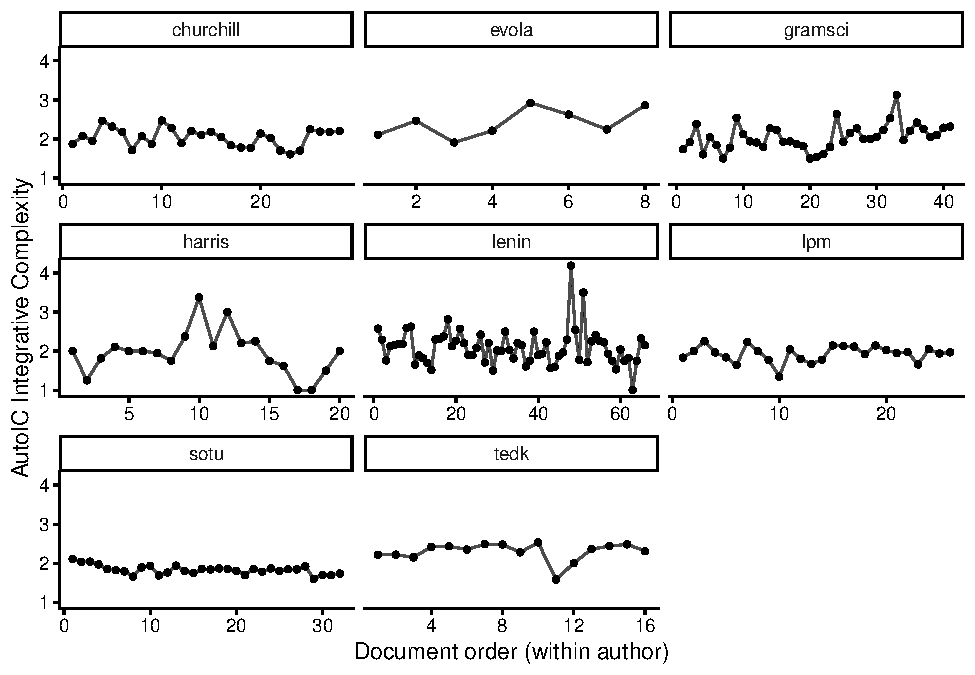
\includegraphics[keepaspectratio]{Thesis_files/figure-latex/fig-long-ic-trajectories-1.pdf}}
\caption{\label{fig:fig-long-ic-trajectories}Longitudinal trajectories of integrative complexity by author (document order).}
\end{figure}

\begin{verbatim}
## Longitudinal rows: 237 
## Authors: 8 
## 
## moderate  extreme  violent 
##       86      115       36
\end{verbatim}

\begin{table}[tbp]

\begin{center}
\begin{threeparttable}

\caption{\label{tab:longitudinal-category-models}Longitudinal mixed-effects models testing category differences in trajectories of integrative complexity and justification language.}

\begin{tabular}{lllll}
\toprule
Model & \multicolumn{1}{c}{Term} & \multicolumn{1}{c}{B} & \multicolumn{1}{c}{SE} & \multicolumn{1}{c}{t}\\
\midrule
Justification \textasciitilde{} IC + Time × Category & Integrative Complexity & -0.12 & 0.13 & -0.88\\
Justification \textasciitilde{} IC + Time × Category & Time & 0.00 & 0.01 & -0.19\\
Justification \textasciitilde{} IC + Time × Category & Extreme vs. Moderate & -0.33 & 0.15 & -2.17\\
Justification \textasciitilde{} IC + Time × Category & Violent vs. Moderate & -0.37 & 0.18 & -2.03\\
Justification \textasciitilde{} IC + Time × Category & Time × Extreme & 0.00 & 0.01 & 0.29\\
Justification \textasciitilde{} IC + Time × Category & Time × Violent & -0.01 & 0.03 & -0.23\\
IC \textasciitilde{} Time × Category & Time & 0.00 & 0.00 & -0.67\\
IC \textasciitilde{} Time × Category & Extreme vs. Moderate & 0.21 & 0.09 & 2.24\\
IC \textasciitilde{} Time × Category & Violent vs. Moderate & 0.18 & 0.11 & 1.67\\
IC \textasciitilde{} Time × Category & Time × Extreme & 0.01 & 0.01 & 1.14\\
IC \textasciitilde{} Time × Category & Time × Violent & -0.01 & 0.01 & -0.56\\
\bottomrule
\addlinespace
\end{tabular}

\begin{tablenotes}[para]
\normalsize{\textit{Note.} Models include random intercepts and random slopes for time by author. Moderate manifestos serve as the reference category.}
\end{tablenotes}

\end{threeparttable}
\end{center}

\end{table}

\section{Discussion}\label{discussion}

The present study examined whether linguistic indicators of harm justification and integrative complexity differentiate political manifestos associated with violence. The results provide partial support for the proposed framework.

First, dyadic harm language reliably distinguished moderate from non-moderate manifestos. Both ideologically extreme and violent texts exhibited higher levels of dyadic harm framing, consistent with dyadic morality theory, which posits that moral cognition is structured around agent--patient representations of harm. However, dyadic harm language did not distinguish violent from non-violent extremity, suggesting that such framing reflects ideological radicalization more broadly rather than violence-specific processes.

Second, martyrdom narratives uniquely differentiated violent manifestos. Violent texts exhibited significantly higher levels of martyrdom language, whereas ideologically extreme texts did not differ from moderate texts. This pattern suggests that narratives of sacrifice and moral heroism may play a distinct role in legitimizing violent action.

Third, integrative complexity was negatively associated with violence likelihood. Lower levels of integrative complexity predicted violent manifestos even when controlling for linguistic indicators, consistent with prior research linking reduced cognitive complexity to conflict escalation and extreme decision-making.

At the same time, several hypothesized effects were not supported. Justification for violence and hopelessness did not significantly differentiate manifesto categories. This suggests that justificatory rhetoric may be characteristic of political discourse more generally rather than uniquely associated with violence. Additionally, longitudinal analyses did not reveal systematic within-author changes, indicating that shifts toward violence may not manifest as gradual linguistic or cognitive changes detectable with the present measures.

Taken together, these findings suggest a functional differentiation between linguistic and cognitive predictors: dyadic harm framing characterizes ideological radicalization, martyrdom narratives distinguish violent from non-violent extremity, and integrative complexity constrains whether radical beliefs translate into violent action.

\subsection{Limitations}\label{limitations}

Several limitations should be noted. First, the corpus remains limited in size and heterogeneous in composition. The inclusion of both terrorist manifestos and broader ideological texts increases generalizability but introduces variability in genre, audience, and historical context.

Second, the dictionary-based approach constrains measurement to predefined lexical indicators and may fail to capture more context-dependent or implicit forms of moral justification.

Third, several regression estimates---particularly in logistic and multinomial models---exhibited wide confidence intervals, indicating limited precision and potential instability in effect size estimates.

Finally, the longitudinal analyses may be underpowered or insufficiently sensitive to detect temporal dynamics, particularly given variation in document spacing and contextual shifts across authors.

\subsection{Future Directions}\label{future-directions}

Future research should extend the present findings in several ways. Increasing corpus size and improving category balance would enhance statistical power and estimate stability. Expanding longitudinal datasets with clearer temporal alignment to behavioral outcomes may also improve sensitivity to within-author changes.

Second, integrating dictionary-based methods with more flexible natural language processing approaches (e.g., semantic embeddings, topic modeling) would allow identification of higher-order moral narratives beyond predefined lexical categories.

Third, future work should explicitly model the interaction between representational content and cognitive structure. The present results suggest that linguistic indicators capture moral framing, whereas integrative complexity reflects structural constraints on reasoning. A process-level model integrating these components may better account for when ideological beliefs result in violence.

Finally, extending this approach to other forms of political communication (e.g., speeches, social media) would test the generalizability of these findings and their potential applicability to broader contexts of ideological escalation.

\newpage

\section{References}\label{references}

\phantomsection\label{refs}
\begin{CSLReferences}{1}{0}
\bibitem[\citeproctext]{ref-ballesteros2025pcc}
Ballesteros, M. (2025). \emph{Propositional cognitive complexity} (Master's thesis). Midwestern State University.

\bibitem[\citeproctext]{ref-capelos2025today}
Capelos, T., DaVisio, K., \& Salmela, M. (2025). {``Today i die like jesus christ''}: An analysis of ressentiment in perceptions, motivations and justifications of violent extremist manifestos. \emph{Terrorism and Political Violence}, \emph{37}(8), 1031--1047.

\bibitem[\citeproctext]{ref-conway2014automated}
Conway, L. G., Conway, K. R., Gornick, L. J., \& Houck, S. C. (2014). Automated integrative complexity. \emph{Political Psychology}, \emph{35}(5), 603--624.

\bibitem[\citeproctext]{ref-conway2020validating}
Conway, L. G., Conway, K. R., \& Houck, S. C. (2020). Validating automated integrative complexity: Natural language processing and the donald trump test. \emph{Journal of Social and Political Psychology}, \emph{8}(2), 504--524.

\bibitem[\citeproctext]{ref-ebner2024measuring}
Ebner, J., Kavanagh, C., \& Whitehouse, H. (2024). Measuring socio-psychological drivers of extreme violence in online terrorist manifestos: An alternative linguistic risk assessment model. \emph{Journal of Policing, Intelligence and Counter Terrorism}, \emph{19}(2), 125--143.

\bibitem[\citeproctext]{ref-ebner2025there}
Ebner, J., Kavanagh, C., \& Whitehouse, H. (2025). Is there a language of terrorists? A comparative manifesto analysis. \emph{Studies in Conflict \& Terrorism}, \emph{48}(6), 601--628.

\bibitem[\citeproctext]{ref-schein2018theory}
Schein, C., \& Gray, K. (2018). The theory of dyadic morality: Reinventing moral judgment by redefining harm. \emph{Personality and Social Psychology Review}, \emph{22}(1), 32--70.

\bibitem[\citeproctext]{ref-suedfeld2010cognitive}
Suedfeld, P. (2010). The cognitive processing of politics and politicians: Archival studies of conceptual and integrative complexity. \emph{Journal of Personality}, \emph{78}(6), 1669--1702.

\bibitem[\citeproctext]{ref-suedfeld199227}
Suedfeld, P., Tetlock, P. E., \& Streufert, S. (1992). \emph{27 conceptual/integrative complexity}.

\bibitem[\citeproctext]{ref-whitehouse2018dying}
Whitehouse, H. (2018). Dying for the group: Towards a general theory of extreme self-sacrifice. \emph{Behavioral and Brain Sciences}, \emph{41}, e192.

\end{CSLReferences}

\newpage

\clearpage

\section{Appendix A}\label{appendix-a}

\begin{table}[H]

\begin{center}
\begin{threeparttable}

\caption{\label{tab:group-descriptives}Descriptive statistics for grouped linguistic indicators of harm justification.}

\begin{tabular}{llllll}
\toprule
Marker Group & \multicolumn{1}{c}{Documents} & \multicolumn{1}{c}{Mean} & \multicolumn{1}{c}{SD} & \multicolumn{1}{c}{Min} & \multicolumn{1}{c}{Max}\\
\midrule
Hopelessness & 267 & 4.58 & 4.59 & 0.00 & 31.21\\
Role Model Status & 267 & 0.56 & 0.83 & 0.00 & 5.02\\
Justification For Violence & 267 & 0.31 & 0.71 & 0.00 & 7.58\\
Martyrdom Narrative & 267 & 0.16 & 0.45 & 0.00 & 4.06\\
Dyadic Harm & 267 & 0.13 & 0.33 & 0.00 & 2.62\\
Violent Reference & 267 & 0.09 & 0.45 & 0.00 & 3.92\\
\bottomrule
\addlinespace
\end{tabular}

\begin{tablenotes}[para]
\normalsize{\textit{Note.} Prevalence values represent marker occurrences per 1,000 words. Marker groups aggregate multiple lexical indicators defined in the study's marker dictionary. Document counts indicate the number of manifestos contributing observations to each group.}
\end{tablenotes}

\end{threeparttable}
\end{center}

\end{table}

\newpage

\clearpage

\section{Appendix B}\label{appendix-b}

\begin{table}[H]

\begin{center}
\begin{threeparttable}

\caption{\label{tab:manifesto-model-fit}Model fit statistics for regressions predicting grouped marker prevalence from manifesto category.}

\begin{tabular}{lllll}
\toprule
Outcome & \multicolumn{1}{c}{R2} & \multicolumn{1}{c}{Adj. R2} & \multicolumn{1}{c}{F} & \multicolumn{1}{c}{p}\\
\midrule
Dyadic Harm & 0.06 & 0.06 & 10.47 & < .001\\
Justification & 0.05 & 0.04 & 7.29 & < .001\\
Martyrdom & 0.00 & 0.00 & 0.51 & 0.604\\
Hopelessness & 0.08 & 0.07 & 12.70 & < .001\\
\bottomrule
\addlinespace
\end{tabular}

\begin{tablenotes}[para]
\normalsize{\textit{Note.} R2 = coefficient of determination; Adj. R2 = adjusted coefficient of determination.}
\end{tablenotes}

\end{threeparttable}
\end{center}

\end{table}


\end{document}
